The ATLAS experiment, in its current form, was first proposed in 1994~\cite{atlas_technical_proposal}, with official funding from CERN member states following in 1995. Construction began in 2003 and was completed in 2008. ATLAS is the largest of the LHC's detectors, measuring 46 meters in length, 25 meters in diameter, and weighing over 7,000 tonnes. It has a symmetric, cylindrical geometry designed to provide nearly full solid-angle coverage about the collision point. The detector is made up of several subsystems arranged as concentric cylindrical layers aligned with the beam pipe. These are further divided into three main regions: the central barrel and two endcaps at either end.

The innermost component of ATLAS is the Inner Detector (ID), which is responsible for tracking charged particles and reconstructing the primary vertex (PV). The ID consists of three technologies: the high-granularity silicon pixel detector situated closest to the interaction point, followed by the Semiconductor Tracker (SCT), and finally the Transition Radiation Tracker (TRT). Surrounding the ID is the calorimeter system, split into the electromagnetic calorimeter, which measures particles like electrons and photons, and the hadronic calorimeter, which captures energy from hadrons such as pions and neutrons. The outermost subsystem is the muon spectrometer, which identifies and measures the momentum of muons, the only charged particles capable of penetrating the entire detector.
The ID is explained in more detail in Section~\ref{sec:atlas_id}, the calorimeter system in Section~\ref{sec:atlas_calorimeter}, and the muon spectrometer in Section~\ref{sec:atlas_muon}. The entire ATLAS detector can be seen in Figure~\ref{fig:atlas_detector}.

\begin{figure}[pht]
    \centering
    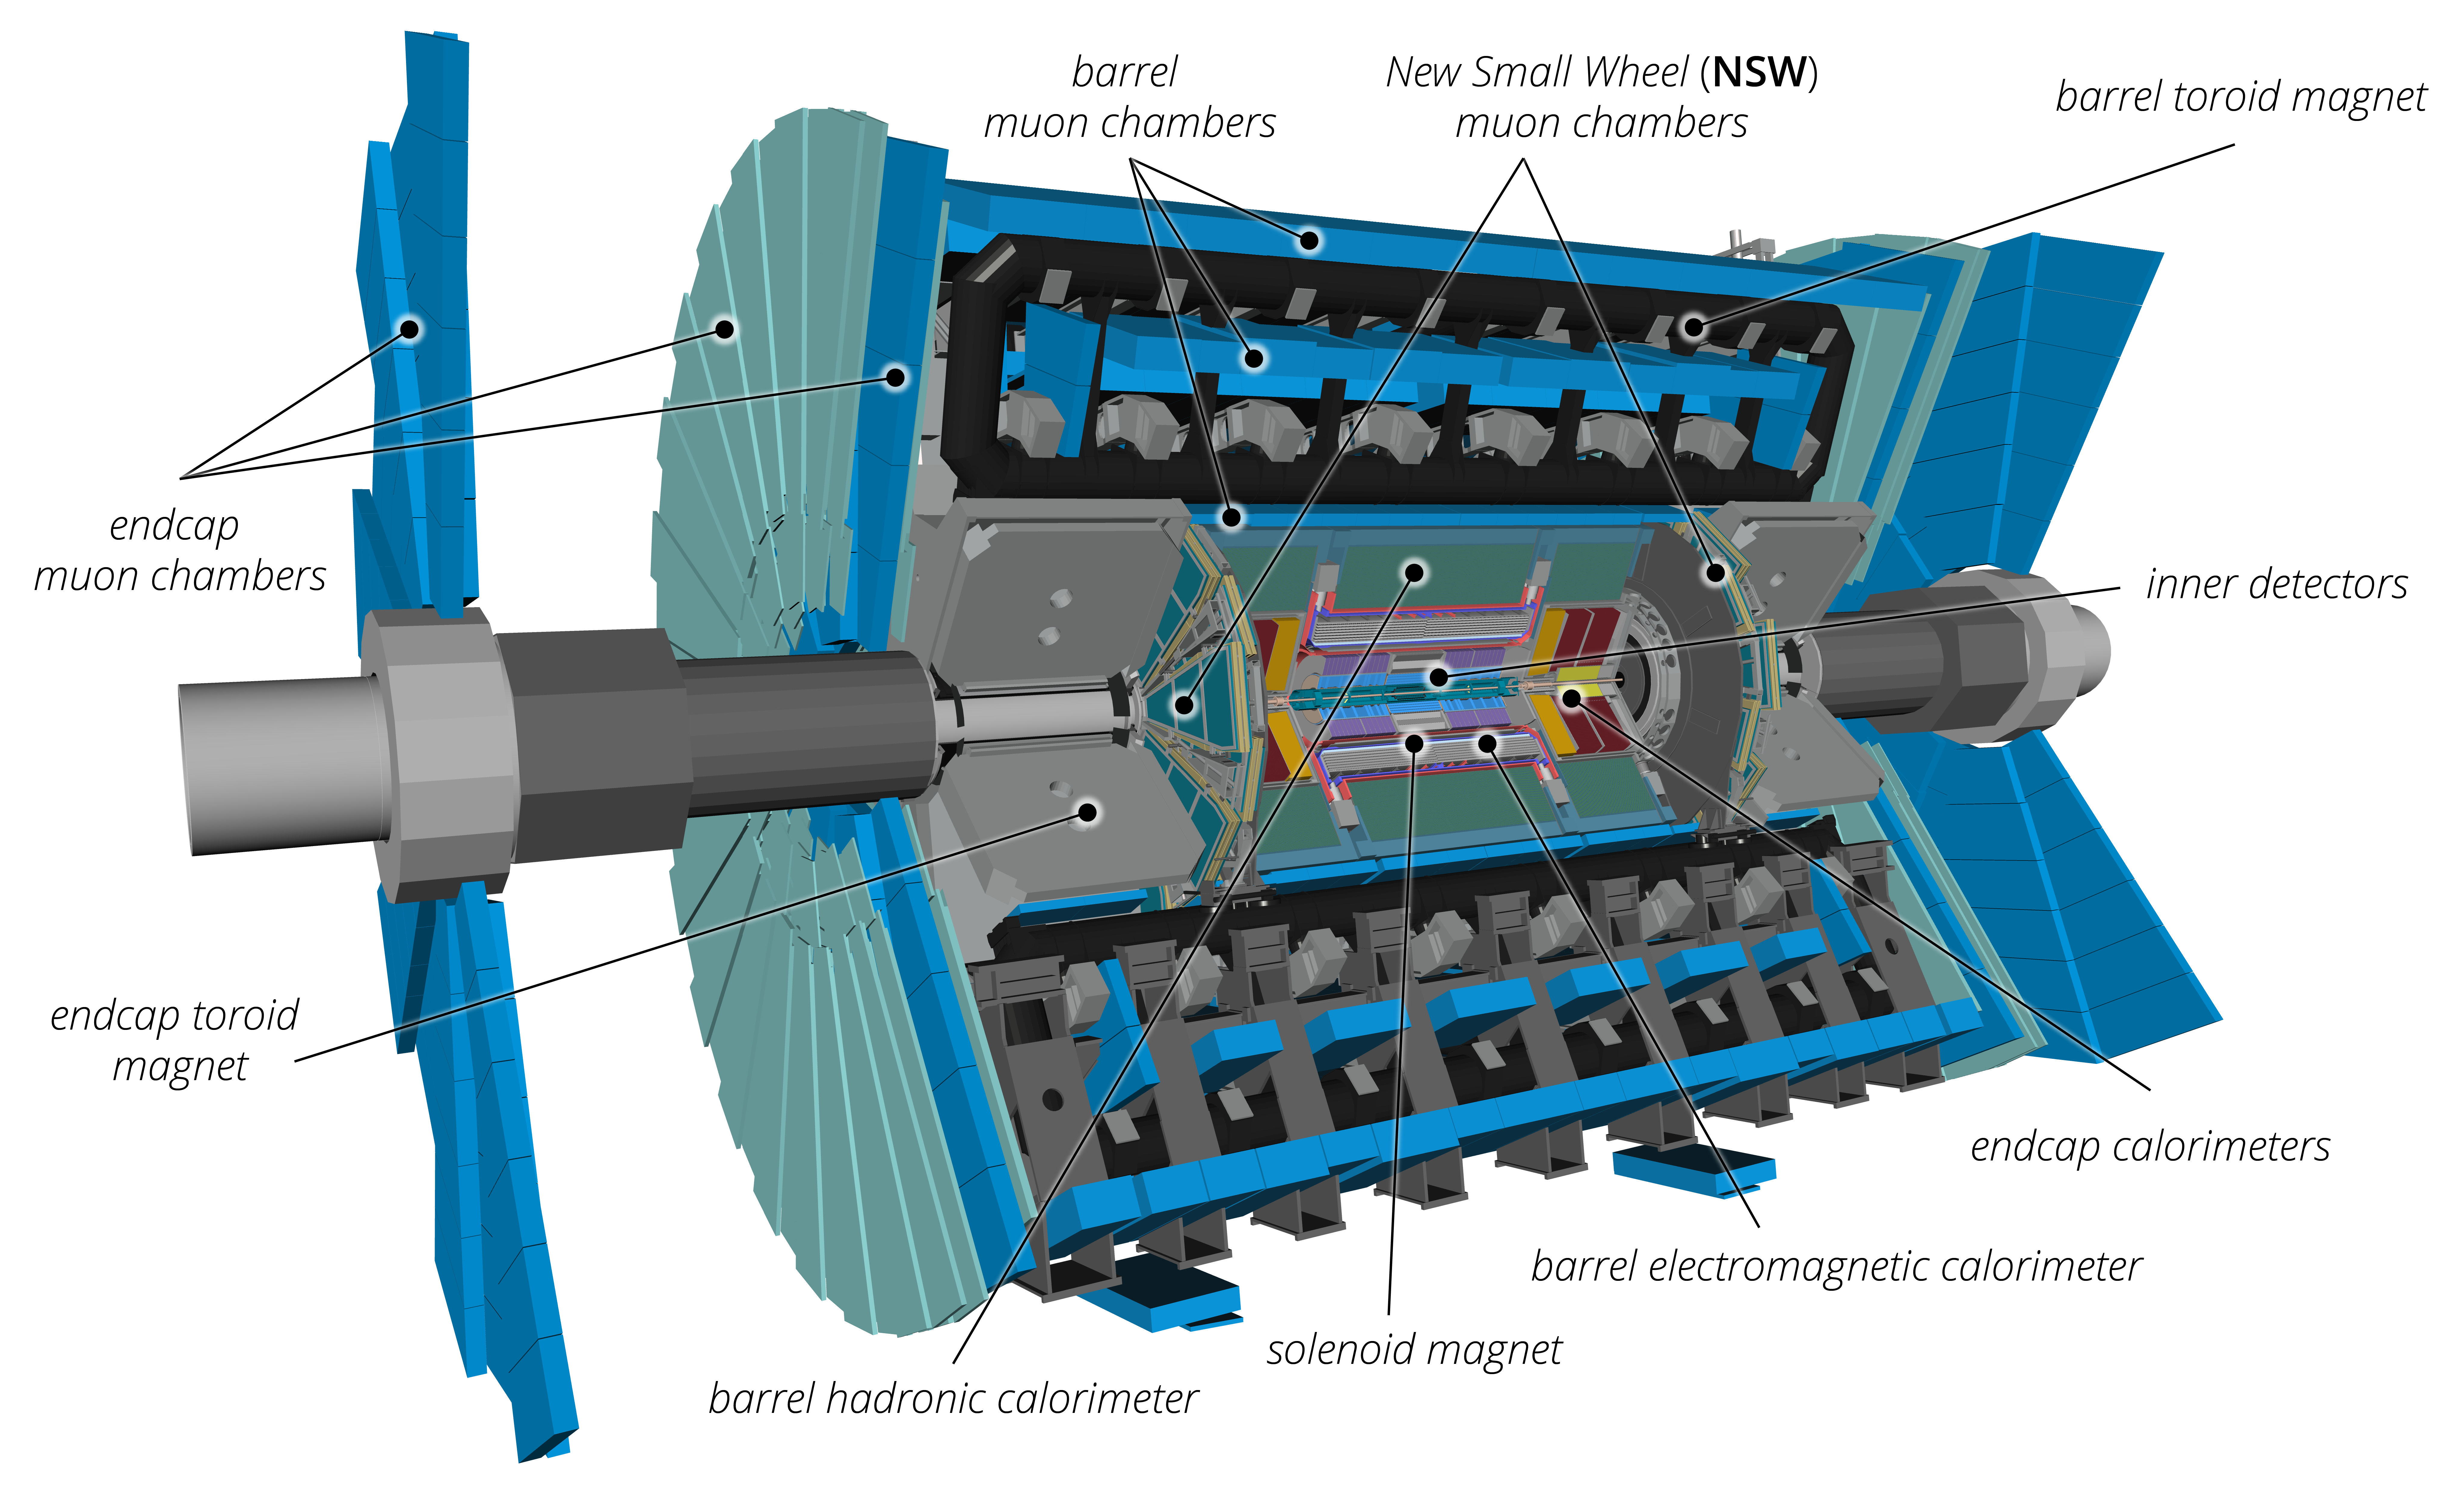
\includegraphics[width=0.9\textwidth]{figures/atlas/atlas_detector.png}
    \caption{Shown is ATLAS with its Run3 detector configuration. The inner detectors are seen in the middle of the figure, followed by the calorimeters, and finally by the muon spectrometer. Taken from~\cite{atlas_figure}}\label{fig:atlas_detector}
\end{figure}